\documentclass{article}
\usepackage[T1]{fontenc}
\usepackage{lmodern}
\usepackage{graphicx}
\usepackage{amsmath,amssymb}
\usepackage[a4paper,margin=2cm]{geometry}
\usepackage[absolute,overlay]{textpos}
\setlength{\TPHorizModule}{1mm}
\setlength{\TPVertModule}{1mm}
\usepackage[indonesian]{babel}
\usepackage{hyperref}
\setlength{\emergencystretch}{2em}
% unit: Halaman 5

\begin{document}

% === Halaman 5 (python/native) ===

5

1.    Chipertext-only attack


Kriptanalis hanya memiliki cipherteks saja. Ini serangan paling sulit karena 

informasi yang diperoleh hanya sedikit (cipherteks saja).


Teknik yang digunakan: exhaustive key search, terkaan, metode analisis 

frekuensi, dsb. 

Diberikan: C1 = Ek(P1), C2 = Ek(P2), …, Ci = Ek(Pi) 

             Deduksi:    P1, P2, …, Pi atau k untuk mendapatkan 



     Pi+1 dari Ci+1 = Ek(Pi+1). 


Sumber: https://www.hackers-arise.com/post/2019/04/30/cryptography-basics-part-

2-attack-models-for-cryptanalysis

% deskripsi: gambar native xref 46
\noindent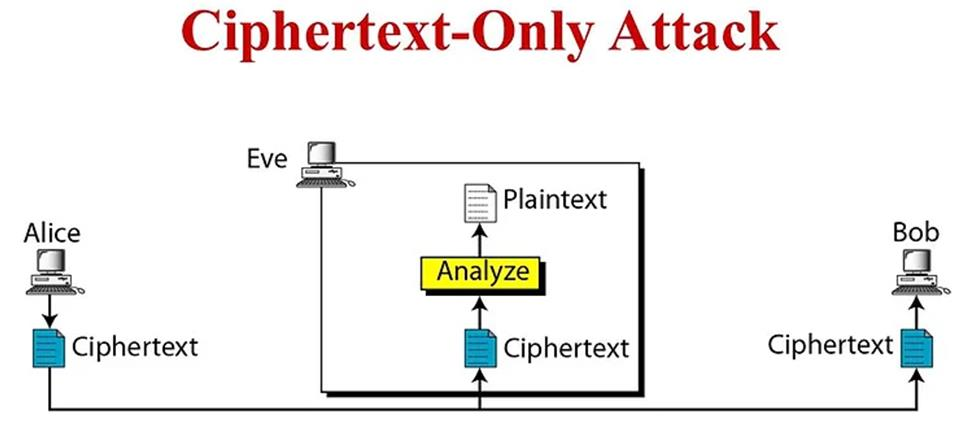
\includegraphics[width=0.85\textwidth]{../../images/python/page_005_img_01.jpeg}

\end{document}
